\begin{figure}[H] 
  \begin{subfigure}[b]{0.5\linewidth}
    \centering
    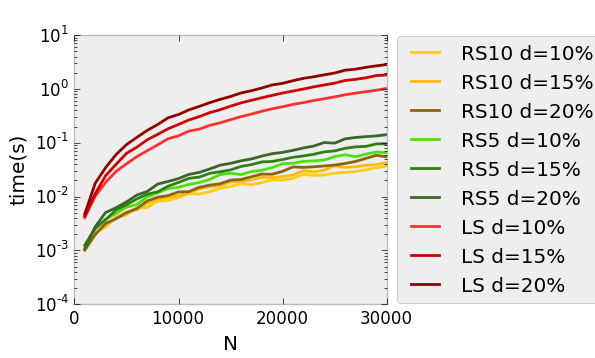
\includegraphics[width=0.9\linewidth]{Pictures/unif_ls_rs_t} 
    %\caption{$N=10$} 
    \label{fig:unif_ls_rs_t} 
    \vspace{4ex}
  \end{subfigure}%% 
  \begin{subfigure}[b]{0.5\linewidth}
    \centering
    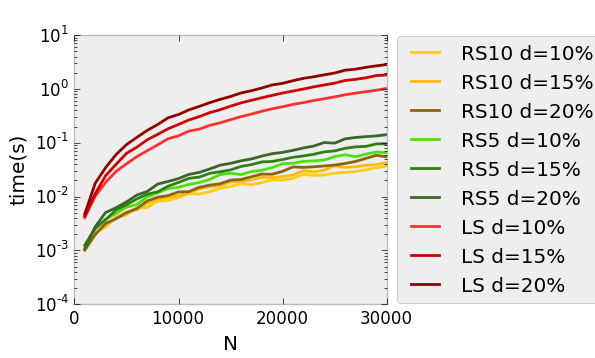
\includegraphics[width=0.9\linewidth]{Pictures/unif_ls_rs_t} 
    %\caption{$N=20$} 
    \label{fig:clus_ls_rs_t} 
    \vspace{4ex}
  \end{subfigure}
  \caption{CPU-time for both random sample algorithms on uniform points(left) and clustered points (right). The red lines represent the control group (line sweep), the green lines represent the 1/5th sampling and the yellow lines represent the 1/10th sampling}
  \label{fig:ls_rs_t} 
\end{figure}

